\documentclass[10pt,letterpaper]{article}

\usepackage{pslatex}
\usepackage{apacite}
\usepackage[utf8]{inputenc}
\usepackage[T1]{fontenc}
\usepackage{lmodern}
\usepackage{multicol}
\usepackage{amsmath}
\usepackage{amssymb}
\usepackage{enumitem}
\numberwithin{equation}{section}
\usepackage{algorithm}
\usepackage{algorithmic}
\usepackage{graphicx}
\usepackage{float}
\usepackage{moreverb}
\usepackage{url}
\usepackage{subcaption}
\setlength\parindent{0pt}
\usepackage{bbm}
\usepackage{booktabs}
\usepackage{longtable}
\usepackage{array}
\usepackage{multirow}
\usepackage[table]{xcolor}
\usepackage{wrapfig}
\usepackage{colortbl}
\usepackage{pdflscape}
\usepackage{tabu}
\usepackage{threeparttable}
\usepackage{threeparttablex}
\usepackage[normalem]{ulem}
\usepackage{makecell}
\usepackage{breakcites}
\usepackage[htt]{hyphenat}
\usepackage{fancyvrb}
\usepackage{algorithm}
\usepackage{algorithmic}
\usepackage{listingsutf8}
\usepackage{color}
\usepackage[margin=1in]{geometry}
\usepackage{hyperref}

\title{{\huge \bf Semantic segmentation for mapping hockey broadcast images in 2D plan}}
 
\author{{\bf Philippe Blouin-Leclerc and Stéphane Caron} \\ {Laval University} \\
{\{philippe.blouin-leclerc.1, stephane.caron.9\}}@ulaval.ca}
  
\date{May 10th 2019}

\begin{document}
\maketitle

\begin{multicols}{2}

\begin{abstract}
Explain the objective of the project. All the codes that aimed to realized that project and that article are hosted on that GitHub \href{https://github.com/stecaron/glo-7030-projet}{repository}.
\end{abstract}


\section{Introduction}

Computer vision is a growing field that changed the faces of many applications in robotic, security or even health sectors. Another field that is currently having more and more interests in such computer vision applications is the sports analytics. The professionnal sports clubs are using analytics and data to understand as more as they can the game and the performances of their players and their opponents. To increase that understanding, you often need a bunch of experts analyzing a bunch of data. Computer vision is well suited to extract that data because it allows the detection of many events simultaneously, which otherwise may have been done by many humans. In order to extract that data properly, it's way more interesting to map those events on the field (or the ice). To do so, it's often necessary to understand the general representation of the moment (or the image), which could be done by a computer vision task called semantic segmentation.
\\
In his work, \cite{Homayounfar} present a methodology where he uses different cues on the field such as lines, corners, circles and so on to train another model that position the field in a 2 dimensionnal plan. In our project, we tried to improve the cues detection technic by training different semantic segmentation models and gain insights on how to train such models. The next step following that project will be to also use that representation in order to map players into a 2 dimensionnal plan.
\\
In the next section, we will start by giving some background about the task of semantic segmentation (section \ref{sec:background}), then we'll present our methodology (section \ref{sec:methodology}), the dataset we used for our experiments (section \ref{sec:dataset}), the results we had (section \ref{sec:results}) and finally a short conclusion (section \ref{sec:conclusion}).

 


\section{Proposed approach}


Explain our approach to map broadcast images.


\section{Datasets}

\subsection{Dataset creation}
We applied the methodology described earlier to hockey broadcast images. We generated our dataset, which contains images (inputs) and masks (outputs), by ourselves. To do so, we annotated a total of 43 NHL broadcast images. For the annotation part, we used an open source tool called \href{https://github.com/opencv/cvat}{cvat tool}. That tool allowed us to draw polygons around our labels and then associate a class to each pixels in the image.

To choose our labels, we used an iterative approach where we first used our judgment to decide arbitrary categories (ex: ice, crowd, corners, horizontal lines, vertical lines). After that, we used one single image and tried to fit a model using those labels. We then noticed the bahviour of the model regarding those categories and adapted them. For example, we noticed the corners, the horizontal and vertical lines such as the board were difficult to distinguish for the model. As such, we decided to merge them and use one single category called "board". Here are the \textbf{9 categories} we selected at the end: ice, boards, crowd, red line, blue lines, goal lines, circles in end zone, circles in neutral zone and dots. The figure \ref{fig:labeling} is an example of image we extracted and then labeled using our 9 categories.

\begin{figure}[H]
	\centering
	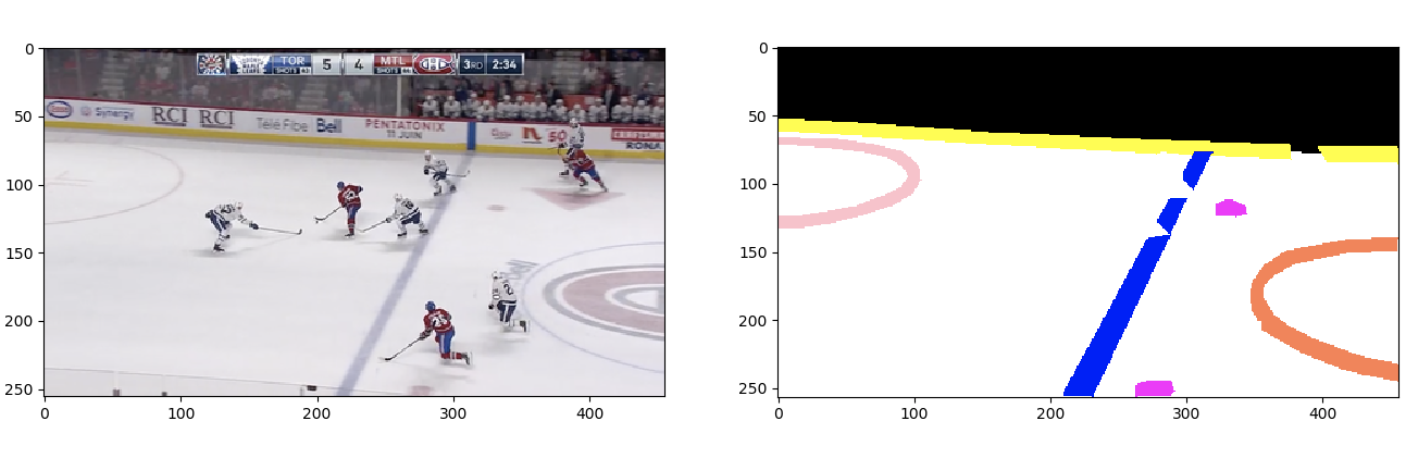
\includegraphics[width=8cm, height=4cm]{figures/labeling-example.png}
	\caption{Example of extracted image (left) and the labeling output (right) using the 9 categories.}
	\label{fig:labeling}
\end{figure}

In the methodology section, we mentionned we had a class imbalance problem. In that section, we tackled this problem by adapting the loss. In the labeling task, we also tackled that class imbalance problem by subjectively drawing larger polygons for rare categories such as dots or circles.



\section{Experiments}


Talk about the task we tried to achieve. Present the resultats and some examples.


\section{Conclusion}

In conclusion, we can first say that we need more images. The lack of images is even more problematic for a non pre-trained model such as the U-Net model. We can also say that a pre-trained model seems to be a must in our learning task, even if we could have a larger dataset. After a lot of training attempts, we also noticed that those can of models seems to learn slowly and over a long period of time. \\
The next steps would be to extract more images. Also, because the pre-trained model was quite successful, we may need to put more focus on using a more specific encoder for that task. In the same idea, we may need to put more efforts on the decoder part of the model, which can hardly be pre-trained in our case. Finally, if we are able to build a adequate semantic segmentation model, we could then use that model to map our images into a 2 dimensional plan.


\nocite{hastie01statisticallearning}

\bibliographystyle{apacite}

\setlength{\bibleftmargin}{.125in}
\setlength{\bibindent}{-\bibleftmargin}

\bibliography{bibliography}

\end{multicols}

\end{document}